\section{Single-State NEVPT}

Let $\Psi_m^{(0)}$ be a zero-order CASCI wavefunction
\beq
\Psi_m^{(0)} = \sumidx{I \in \mbox{\tiny CAS}} C_{I,m} \ket{I}
\eeq
obtained diagonalizing $\ham$ inside the CAS
\beq
\proj{\mbox{\tiny CAS}}\ham\proj{\mbox{\tiny CAS}}\ket{\Psi_m^{(0)}} = E_m^{(0)} \ket{\Psi_m^{(0)}}
\eeq
where $\proj{\mbox{\tiny CAS}}$ is the projector inside the CASCI space. 

We can define perturbers in NEVPT as zero-order wavefunctions of the outer
space (external to CAS) where $k$ electrons are removed from the inactive
part and added to the valence part. If we decompose the zero-order CASCI
wavefunction as an antisymmetrized product of an inactive part (made of both
core and virtual orbitals) with $n_c$ electrons, and a valence part (made of
active orbitals) with $n_v$ electrons
\beq
\ket{\Psi_m^{(0)}} = \ket{\Phi_c \Psi_m^v}
\eeq
then the perturber wavefunctions can be expressed as
\beq
\ket{\Psi_{l,\mu}^{k}} = \ket{\Phi_l^{-k} \Psi_{\mu}^{v+k}}
\eeq
where $l$ is a collective index that describes the orbitals involved in the
operation and $\mu$ an enumerator index for the different wavefunctions. At
second order of perturbation $-2 \le k \le 2$.  

A graphical representation of the excitation scheme for NEVPT can be seen in
Fig. \ref{fig:classes}

\begin{center}
\begin{figure}[ht]
\begin{center}
\includegraphics[width=9cm,angle=270]{03_nevpt/images/classes.ps}
\end{center}
\caption{\footnotesize The eight excitation classes defining the perturber
functions in NEVPT.}
\label{fig:classes}
\end{figure}
\end{center}


The perturbers functions span a space of determinants with the same inactive
part $\Phi_l^{-k}$ and all the possible valence parts $\Psi_I^{+k}$. These
spaces are denoted as $S_l^k$
\beq
S_{l}^{k} \equiv \left\{ \Phi_l^{-k} \Psi_I^{+k} \right\}
\eeq
Perturbers will be defined in these spaces. If the full dimensionality
is exploited, the resulting approach is called \textit{totally
uncontracted}. The perturbers and their energies can be obtained by
diagonalizing the Hamiltonian inside each space
\beq
\label{eqn:teoria1_1}
\proj{S_l^k}\ham\proj{S_l^k} \ket{\Phi_l^{-k} \Psi_{\mu}^{v+k}} = E_{l,\mu}
\ket{\Phi_l^{-k} \Psi_{\mu}^{v+k}}
\eeq
however, this procedure is impractical given its high computational cost.
For each $S_l^k$ space, a diagonalization of the true Hamiltonian must be performed.

We can improve the computational asset by introducing a modified
Hamiltonian, proposed by Dyall\cite{jcp-102-4909-1995}
\beqa
\ham^D &=& \ham^D_i + \ham^D_v + C \\
\ham^D_i &=& \sum_{i}^{\mbox{\tiny core}} \epsilon_i E_{ii} +
\sum_r^{\mbox{\tiny virt}} \epsilon_r E_{rr} \\
\ham^D_v &=& \sum_{ab}^{\mbox{\tiny act}} h_{ab}^{\mbox{\tiny eff}} E_{ab} +
\frac{1}{2} \sum_{abcd}^{\mbox{\tiny act}} \integral{ab}{cd} \left( E_{ac}
E_{bd} - \delta_{bc} E_{ad} \right) \\
C &=& 2 \sum_{i}^{\mbox{\tiny core}} h_{ii} + \sum_{ij}^{\mbox{\tiny core}}
\left( 2 \integral{ij}{ij} - \integral{ij}{ji} \right) - 2
\sum_{i}^{\mbox{\tiny core}} \epsilon_i
\eeqa
where labels $i,j,\ldots$, $a,b,\ldots$, $r,s,\ldots$ denote core, active
and virtual orbitals respectively, and this convention will be retained
hereafter, $\epsilon_i$ and $\epsilon_r$ are the orbital energies of the
involved orbitals, and $E_{mn}$ operators are the spin-traced operators
$\constr{m\alpha}\destr{n\alpha} + \constr{m\beta}\destr{n\beta}$. These
operators commute with $S^2$ and $S_z$, therefore the application of these
operators on a spin-pure function produces again a spin-pure function.
Finally, the $h_{ab}^{\mbox{\tiny eff}}$ matrix evaluates as
\beq
h_{ab}^{\mbox{\tiny eff}} =  h_{ab} + \sum_j \left( 2 \integral{aj}{bj} -
\integral{aj}{jb} \right)
\eeq

$\ham^D$ behaves like the true Hamiltonian inside the CAS space, having the
same eigenvalues and eigenvectors of the true Hamiltonian projected onto the
CAS space. Also, given the decomposition for the wavefunction defined
before, the action of the Dyall's Hamiltonian can be partitioned
\beq
\ham^D \ket{\Phi_l^{-k} \Psi_{\mu}^{v+k}} = E_{l,\mu}^{k} \ket{\Phi_l^{-k}
\Psi_{\mu}^{v+k}} 
\eeq
stripping out the constant contribution of the inactive part and leaving a
subsystem to be solved for the valence part
\beq
\ham^D_v \ket{\Psi_{\mu}^{v+k}} = E_{\mu}^{k} \ket{\Psi_{\mu}^{v+k}} 
\eeq
The total energy $E_{l,\mu}^{k}$ is the sum of $E_{\mu}^{k}$ and the 
energies of the orbitals involved in the definition of the inactive part
$\Phi_l^{-k}$. This introduces the possibility to perform a single
diagonalization of the valence Dyall's Hamiltonian on the CASCI zero-order
wavefunction and evaluate the perturber energies using the property depicted
above.

\subsection*{Strongly Contracted approach}

A possible choice in the development of the NEVPT approach is to choose a
single function for each space $S_l^k$, leading to the \textit{Strongly
Contracted (SC)} scheme. A set of perturbative operators are used to produce a
single function for each space, according to the following definition
\beq
\Psi_l^k = \proj{S_l^k} \ham \Psi_m^{(0)}
\eeq
where $\proj{S_l^k}$ is the projector onto the subspace $S_l^k$. The same
result can be obtained by applying a specific part of the Hamiltonian to the
zero-order wavefunction
\beq
\Psi_l^k = V_l^k \Psi_m^{(0)}
\eeq

For each space, an appropriate operator can be devised
\beqa
V_{ijrs}^{0} &=& \gamma_{ij} \gamma_{rs} \left( \integral{rs}{ij} E_{ri} E_{sj} + \integral{rs}{ji} E_{si} E_{rj} \right) \quad i \le j, r \le s \\
V_{rsi}^{-1} &=& \gamma_{rs} \sum_a \left( \integral{rs}{ia} E_{ri} E_{sa} + \integral{sr}{ia} E_{si} E_{ra} \right) \quad  r \le s \\
V_{ijr}^{1} &=& \gamma_{ij} \sum_a \left( \integral{ra}{ji} E_{rj} E_{ai} + \integral{ra}{ij} E_{ri} E_{aj} \right) \quad  i \le j \\
V_{rs}^{-2} &=& \gamma_{rs} \sum_{ab} \integral{rs}{ba} E_{rb} E_{sa} \quad  r \le s \\
V_{ij}^{2} &=& \gamma_{ij} \sum_{ab} \integral{ba}{ij} E_{bi} E_{aj} \quad  i \le j \\
V_{ir}^{0} &=& \sum_{ab} \left( \integral{ra}{ib} E_{ri} E_{ab} + \integral{ra}{bi} E_{ai} E_{rb} \right) + h_{ri}^{\mbox{\tiny eff}} E_{ri} \\
V_r^{-1} &=& \sum_{abc} \integral{ra}{bc} E_{rb} E_{ac} + \sum_{a} h_{ra}^{\mbox{\tiny eff'}} E_{ra} \\
V_i^{1} &=& \sum_{abc} \integral{ba}{ic} E_{bi} E_{ac} + \sum_{a} h_{ai}^{\mbox{\tiny eff}} E_{ai}
\eeqa
where $\gamma_{mn} = 1 - \half \delta_{mn}$.

Auxiliary matrixes have been also defined as
\beqa
h_{mn}^{\mbox{\tiny eff}} &=& h_{mn} + \sum_j \left( 2 \integral{mj}{nj} -
\integral{mj}{jn} \right) \\
h_{mn}^{\mbox{\tiny eff'}} &=& h_{mn}^{\mbox{\tiny eff}} - \sum_b
\integral{mb}{bn}
\eeqa
The perturber functions are not normalized. The norm of these functions
\beq
N_l^k = \integral{\Psi_l^k}{\Psi_l^k} = \braket{\Psi_m^{(0)}}{
\left(V_l^k\right)^+  V_l^k }{\Psi_m^{(0)}}
\eeq
plays an important role in the Strongly Contracted development. The values
of the norms for each function are
\beqa
N_{ijrs}^{0} &=& 4 \gamma_{ij} \gamma_{rs} \left( \integral{rs}{ij}^2 + \integral{rs}{ji}^2 - \integral{rs}{ij}\integral{rs}{ji} \right) \\
%
N_{rsi}^{-1} &=& \gamma_{rs} \sum_{ab} \left[ 2 \left(\integral{rs}{ib}\integral{rs}{ia} + \integral{sr}{ib}\integral{sr}{ia} \right) \right. \nonumber \\
& & \left. - \integral{rs}{ib} \integral{sr}{ia} - \integral{sr}{ib} \integral{rs}{ia}\right] R_{ba}^{(1)} \\
%
N_{ijr}^{1} &=& \gamma_{ij} \sum_{ab} \left[ 2 \left(\integral{rb}{ji}\integral{ra}{ji} + \integral{rb}{ij}\integral{ra}{ij} \right) \right. \nonumber \\
& & \left. - \integral{rb}{ji} \integral{ra}{ij} - \integral{rb}{ij}
\integral{ra}{ji}\right] \tilde{R}_{ba}^{(1)} \\
N_{rs}^{-2} &=& \gamma_{rs} \sum_{abcd} \integral{rs}{ba} \integral{rs}{dc} R_{abcd}^{(2)} \\
%
N_{ij}^{2} &=& \gamma_{ij} \sum_{abcd} \integral{ba}{ij} \integral{dc}{ij} \tilde{R}_{abcd}^{(2)} 
\eeqa
\beqa
N_{ir}^{0} &=& \sum_{abcd} \left[ \left( 2
\integral{ra}{ib}\integral{rc}{id} - \integral{ra}{ib}\integral{rc}{di} - \integral{ra}{bi} \integral{rc}{id} \right) \braket{\Psi_m^{(0)}}{E_{ba}E_{cd}}{\Psi_m^{(0)}} \right. \nonumber \\
& & \left. + \integral{ra}{bi} \integral{rc}{di} \left( \braket{\Psi_m^{(0)}}{E_{bd}\tilde{E}_{ac}}{\Psi_m^{(0)}} + \delta_{ab} R_{ba}^{(1)}\right) \right] \nonumber\\
& & + 2 \sum_{ab} \left(2 \integral{ra}{ib} - \integral{ra}{bi} \right) h_{ri}^{\mbox{\tiny eff}} R_{ba}^{(1)} + 2 \left( h_{ri}^{\mbox{\tiny eff}}\right)^2 \\
%
N_{r}^{-1} &=& \sum_{abcdef} \integral{rd}{ef} \integral{ra}{bc} \braket{\Psi_m^{(0)}}{E_{fd}E_{eb}E_{ac}}{\Psi_m^{(0)}} \nonumber \\
&& + 2 \sum_{abcd} \integral{ra}{bc} h_{ra}^{\mbox{\tiny eff'}} \braket{\Psi_m^{(0)}}{E_{ca}E_{bd}}{\Psi_m^{(0)}} \nonumber \\
&&+ \sum_{ab} h_{ra}^{\mbox{\tiny eff'}} h_{rb}^{\mbox{\tiny eff'}} R_{ba}^{(1)} \\
%
N_{i}^{1} &=& \sum_{abcdef} \integral{ed}{if} \integral{ba}{ic} \braket{\Psi_m^{(0)}}{E_{fd}\tilde{E}_{eb}E_{ac}}{\Psi_m^{(0)}} \nonumber \\
&&+ 2 \sum_{abcd} \integral{ba}{ic} h_{di}^{\mbox{\tiny eff}} \braket{\Psi_m^{(0)}}{E_{ca}\tilde{E}_{bd}}{\Psi_m^{(0)}} \nonumber\\
&&+ \sum_{ab} h_{ai}^{\mbox{\tiny eff}} h_{bi}^{\mbox{\tiny eff}} \tilde{R}_{ba}^{(1)}
\eeqa
To evaluate these norms, the spinless density matrix of rank not higher than
three between the $\Psi_m^{(0)}$ functions are needed.  A short notation has
been used for the hole density matrixes
\beqa
\tilde{R}_{ab}^{(1)} &=& 2 \delta_{ab} - R_{ba}^{(1)} \\
\tilde{R}_{abcd}^{(2)} &=& R_{abcd}^{(2)} + \delta_{ad} R_{cb}^{(1)} + \delta_{bc} R_{da}^{(1)} - 2 \delta_{ac} R_{db}^{(1)} \\
& & - 2 \delta_{bd} R_{ca}^{(1)} - 2 \delta_{ad} \delta_{bc} + 4 \delta_{ca} \delta_{db}
\eeqa
and for the operator $\tilde{E}_{ab} = 2 \delta_{ab} - E_{ba}$

An important property of the $\Psi_{l}^{k}$ is that any other function of
the space $S_l^k$ which is orthogonal to  $\Psi_{l}^{k}$ do not interact
with the zero-order wavefunction through the true Hamiltonian. It is
possible to use the  $\Psi_{l}^{k}$ functions as a basis set for the
expansion of the first-order correction to the wavefunction, and also for
the expression of the zero-order Hamiltonian by means of a spectral
decomposition
\beq
\ham_0 = \sum_{lk} \ket{ {\Psi_{l}^{k}}' } E_{l}^{k} \bra{ {\Psi_{l}^{k}}' } +
\sum_{m}  \ket{\Psi_{m}^{(0)}} E_{m}^{(0)} \bra{\Psi_{m}^{(0)}}
\eeq
where $\ket{ {\Psi_{l}^{k}}' }$ are the normalized $\ket{ \Psi_{l}^{k} }$. 

The expression for the first-order correction to the wavefunction is
therefore
\beqa
\Psi_m^{(1)} &=& \sum_{kl} \ket{{\Psi_{l}^{k}}'}
\frac{\braket{{\Psi_{l}^{k}}'}{\ham}{\Psi_{m}^{(0)}}}{E_m^{(0)} - E_{l}^{k}} \\
&=& \sum_{kl} \ket{{\Psi_{l}^{k}}'} \frac{\sqrt{N_l^k}}{E_{m}^{(0)} - E_{l}^{k}} 
\eeqa
and for the energy is
\beq
E_{m}^{(2)} = \sum_{kl} \frac{\braket{{\Psi_{l}^{k}}'}{\ham}{\Psi_{m}^{(0)}}^2} {E_m^{(0)} - E_{l}^{k}} = \sum_{kl} \frac{N_l^k}{E_m^{(0)} - E_{l}^{k}}
\eeq
however, we still miss a definition of the perturber energies $E_l^k$.
These energies can be defined in a computationally advantageous approach, by
means of the Dyall's Hamiltonian.
\beq
E_{l}^{k} = \frac{1}{N_l^k} \braket{\Psi_{l}^{k}}{\ham^D}{\Psi_{l}^{k}}
\eeq
which leads to
\beqa
N_{l}^{k} E_{l}^{k} &=& \braket{\Psi_{m}^{(0)}}{{V_{l}^{k}}^{+} \ham^D
V_{l}^{k}}{\Psi_{m}^{(0)}} \\
 &=& \braket{\Psi_{m}^{(0)}}{{V_{l}^{k}}^{+} V_{l}^{k}
\ham^D}{\Psi_{m}^{(0)}} + \braket{\Psi_{m}^{(0)}}{{V_{l}^{k}}^{+}
\commut{\ham^D}{V_{l}^{k}} }{\Psi_{m}^{(0)}} 
\eeqa
Developing the braket and extracting the inactive part of the Dyall's
Hamiltonian we obtain
\beq
E_{l}^{k} = E_m^{(0)} + \Delta \epsilon_l + \frac{1}{N_l^k}
\braket{\Psi_{m}^{(0)}}{{V_{l}^{k}}^{+}
\commut{\ham_v}{V_{l}^{k}} }{\Psi_{m}^{(0)}}
\eeq
with $\Delta \epsilon_l$ is the sum of the orbital energies of the newly
occupied virtual orbitals minus the orbital energies of the unoccupied core
orbitals. 

The term that still need to be evaluated is the braket involving the
commutator. After development of each $V$ operator and substitution, we
obtain the contributions to the energy. Here we present the result for
$V_{rsi}^{(-1)}$:
\beqa
\braket{\Psi_{m}^{(0)}}{V_{rsi}^{(-1)}
\commut{\ham_v}{V_{rsi}^{(-1)}}}{\Psi_{m}^{(0)}} &=& \gamma_{rs} \sum_{ab}
\left[ 2 \left( \integral{rs}{ia} \integral{rs}{ib} + \integral{sr}{ia}
\integral{sr}{ib} \right) \right. \nonumber \\
&&\left. -\left( \integral{rs}{ia} \integral{sr}{ib} + \integral{sr}{ia}
\integral{rs}{ib}\right) \right] K_{ab} \nonumber \\
\eeqa
where $K_{ab}$ is analogous to a spin-free formulation of the Koopmans
matrix, defined only in the active space
\beqa
\label{eqn:koopmans_matrix}
K_{ab} &=& \half \braket{\Psi_{m}^{(0)}}{E_{as}E_{ir} \commut{\ham_v}{E_{ri}E_{sb}}}{\Psi_{m}^{(0)}} \\
&=& \sum_{c} h_{ac}^{\mbox{\tiny eff}} R_{bc}^{(1)} - \sum_{cde} \integral{cb}{ed} R_{acde}^{(2)} 
\eeqa
The contribution of the $\Psi_{rsi}^{-1}$ is therefore given by
\beq
E_m^{(2)}\left( S_{rsi}^{-1} \right) = - \frac{N_{rsi}^{-1}}{\epsilon_r
+\epsilon_s - \epsilon_i - \epsilon_{rsi}^{-1}}
\eeq
with
\beq
\epsilon_{rsi}^{-1} = \frac{1}{N_l^k}
\braket{\Psi_{m}^{(0)}}{{V_{rsi}^{-1}}^{+}
\commut{\ham_v}{V_{rsi}^{-1}} }{\Psi_{m}^{(0)}}
\eeq

An interesting case is the $V_{ijrs}^{(0)}$ case, which is identical to the
M{\o}ller-Plesset contribution 

\beq
E_m^{(2)}\left( S_{rsij}^{0} \right) = - \frac{N_{rsij}^{0}}{\epsilon_r
+\epsilon_s - \epsilon_i - \epsilon_{j}}
\eeq

NEVPT2 can therefore be seen as a generalized form of MP2 to multireference
wavefunctions, and this result is also found in the completely uncontracted
and Partially Contracted approaches\cite{cpl-317-472-2000}.

The cases involving the $V_{rs}^{-2}$  and $V_{ij}^{2}$ operators require
the knowledge of the three-particles density matrix, and the $V_{r}^{-1}$
and $V_{i}^{1}$ require auxiliary matrixes depending on the four-particles
density matrixes. All these matrixes always involve only the active indexes,
therefore represent only a minor issue for nowadays computers.

\subsection*{Partially Contracted approach}

An alternative approach, named \textit{Partially Contracted
(PC)}, is to use a subspace $\overline{S}_l^k$ of $S_l^k$.
To define this subspace, a set of functions $\Phi$ is generated by means of
the $V_l^k$ operators. These functions must be orthonormalized and purged of
linear dependencies which may arise. The resulting set spans the
$\overline{S}_l^k$ space.

Once the $\overline{S}_l^k$ spaces have been defined, we can obtain a set of
perturbers
\beq
\proj{\overline{S}_l^k}\ham\proj{\overline{S}_l^k} \ket{\Psi_{l\mu}^{k}} =
E_{l,\mu}^{k} \ket{\Psi_{l\mu}^{k}}
\eeq
where we can substitute $\ham$ with $\ham^D$ to simplify the evaluation.
Perturbers are generated by the application of the excitation operators
without contraction. For example, in the case of the $V_{rsi}^{-1}$ operator
\beq
V_{rsi}^{-1} = \gamma_{rs} \sum_a \left( \integral{rs}{ia} E_{ri} E_{sa} + \integral{sr}{ia} E_{si} E_{ra} \right) \quad  r \le s
\eeq
the Partially Contracted approach makes use of functions $\Phi_{risa} =
E_{ri} E_{sa} \Psi_m^{(0)}$ and $\Phi_{risa} = E_{si} E_{ra} \Psi_m^{(0)}$.
We can group these functions in two row vectors $\mathbf{\Phi}_{ris}$ and
$\mathbf{\Phi}_{sir}$ to write the expression of the overlap and $\ham^D$
matrixes
\beq
\integral{\mathbf{\Phi}_{ris}, \mathbf{\Phi}_{sir} }{\mathbf{\Phi}_{ris},
\mathbf{\Phi}_{sir}} = 
\left[ 
\begin{array}{cc}
2 R^{(1)} & - R^{(1)} \\
- R^{(1)} & 2 R^{(1)} 
\end{array}
\right]
\eeq
\beqa
\braket{\mathbf{\Phi}_{ris}, \mathbf{\Phi}_{sir} }{\ham^{D}}{\mathbf{\Phi}_{ris},
\mathbf{\Phi}_{sir}} & = & \left[ 
\begin{array}{cc}
2 \mathbf{K} & - \mathbf{K} \\
- \mathbf{K} & 2 \mathbf{K}
\end{array}
\right] \nonumber \\
&  & + \left( E_m^{(0)} +\epsilon_r +\epsilon_s - \epsilon_i \right)
\left[ 
\begin{array}{cc}
2 \mathbf{R}^{(1)} & - \mathbf{R}^{(1)} \\
- \mathbf{R}^{(1)} & 2 \mathbf{R}^{(1)} 
\end{array}
\right] \nonumber \\
\eeqa
where $\mathbf{R}^{(1)}$ is the one-particle density matrix in the spinless
formulation and the $\mathbf{K}$ matrix is defined as \ref{eqn:koopmans_matrix}
The diagonalization of the $\ham^D$ matrix is quickly obtained diagonalizing
$\mathbf{K}$ in the metric $\mathbf{R}^{(1)}$ to obtain $\mathbf{c}_{\mu}$ coefficients and
$\epsilon_{\mu}$ energies
\beq
\mathbf{K} \mathbf{c}_{\mu} = - \epsilon_{\mu} \mathbf{R}^{(1)} \mathbf{c}_{\mu}
\eeq
to obtain two distinct orthonormal functions
\beqa
\Psi_{ris\mu}^{-1} = \frac{1}{\sqrt{2}} \sum_{a} c_{a \mu} \left( \Phi_{risa} +
\Phi_{sira} \right) \\
{\Psi_{ris\mu}^{-1}}' = \frac{1}{\sqrt{6}} \sum_{a} c_{a \mu} \left( \Phi_{risa} -
\Phi_{sira} \right)
\eeqa
These functions will be used in the evaluation of the interaction with the
zero-order wavefunction. We define
\beqa
\left( rs, \mu i \right) &=& \braket{\Psi_{ris\mu}^{-1}}{\ham}{\Psi_{m}^{(0)}} \\
                         &=& \frac{1}{\sqrt{2}} \sum_{a} \left( \integral{rs}{ia} + \integral{sr}{ia} \right) S_{a \mu}
\eeqa
\beqa
{\left( rs, \mu i \right)}' &=& \braket{{\Psi_{ris\mu}^{-1}}'}{\ham}{\Psi_{m}^{(0)}} \\
                         &=& \sqrt{\frac{3}{2}} \sum_{a} \left( \integral{rs}{ia} - \integral{sr}{ia} \right) S_{a \mu}
\eeqa
where 
\beq
S_{a \mu} = \sum_{a'}  c_{a \mu}^{*} R_{a' a}^{(1)}
\eeq
We can now finally write the contribution for this subspace to the
second-order energy
\beq
E^{(2)}(\overline{S}_{rsi}^{-1}) = - \sum_{\mu} \frac{\left( rs, \mu
i\right)^2 + {\left( rs, \mu 
i\right)'}^2}{\epsilon_r + \epsilon_s - \epsilon_i - \epsilon_{\mu}}
\eeq

